\documentclass{article}
\usepackage[letterpaper]{geometry}
\geometry{verbose,tmargin=1in,bmargin=1in,lmargin=1in,rmargin=1in}

\usepackage[utf8]{inputenc}
\usepackage{amsmath}
\usepackage{float}
\usepackage{listings}
\usepackage{graphicx}
\usepackage{enumitem}

\renewcommand{\baselinestretch}{1.5}

\title{CIS 419/519: Homework 5}
\author{\{Yupeng Li\}}
\date{03.17.2020}

\begin{document}
    \maketitle
    Although the solutions are entirely my own, I consulted with the following people and sources while working on this homework: \textbf{}
    \paragraph{PART1: PROBELM SET}
    \section{Logical Functions with Neural Nets}
    \textbf{(a)} 
    The NAND logic follows a truth table as follows:
    \begin{center}
\begin{tabular}{ c c c }
 $x_0$ & $x_1$ & $H(x)$ \\ 
 0 & 0 & 1 \\  
 0 & 1 & 1 \\  
 1 & 0 & 1 \\
 1 & 1& 0  \\
\end{tabular}
\end{center}

If we use sigmoid as our activation function at the output node, where $\sigma(z) = \frac{1}{1+exp(-z)}$
\\and $H(x) = \sigma(w_0 + w_1 x_0 + w_2 x_2)$, where $w_0 = 40$, and $w_1 = w_2 =  -25$ we would then have:

\begin{center}
\begin{tabular}{ c c c }
 $x_0$ & $x_1$ & $H(x)$\\ 
 0 & 0 & \sigma(40) = 1 \\  
 0 & 1 & \sigma(15) = 1 \\  
 1 & 0 & \sigma(15) = 1 \\
 1 & 1 &  \sigma(-10) = 0 \\
\end{tabular}
\end{center}
\\The neural network that is used to compute this function is the same as in the graph given in the problem set. 

		\begin{figure}[H]
			\caption{Neural network for NAND Logic}
			\centering
			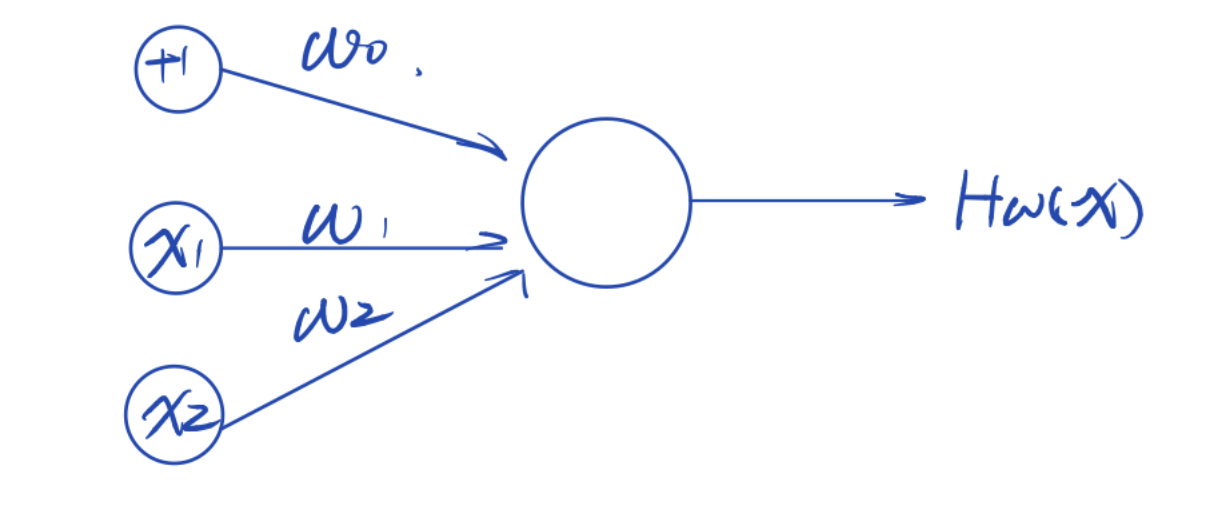
\includegraphics[width=8cm]{HW5_1.jpeg}
		\end{figure}
\\
\textbf{(b)}


    

    
   

        
\end{document}